\chapter{State Consistency}
\label{chp:CONSISTENCY}

\section{Introduction}

A recent article has identified six key challenges of P2P systems: Interest Management, Game Event Dissemination, Non-player Character (NPC) Host
Allocation, Game State Persistency, Cheating Mitigation and Incentive Mechanisms \cite{Fan_deisgn_issues_p2p}. A brief overview of these challenges
will be introduced below.

\begin{figure}[htbp]
 \centering
 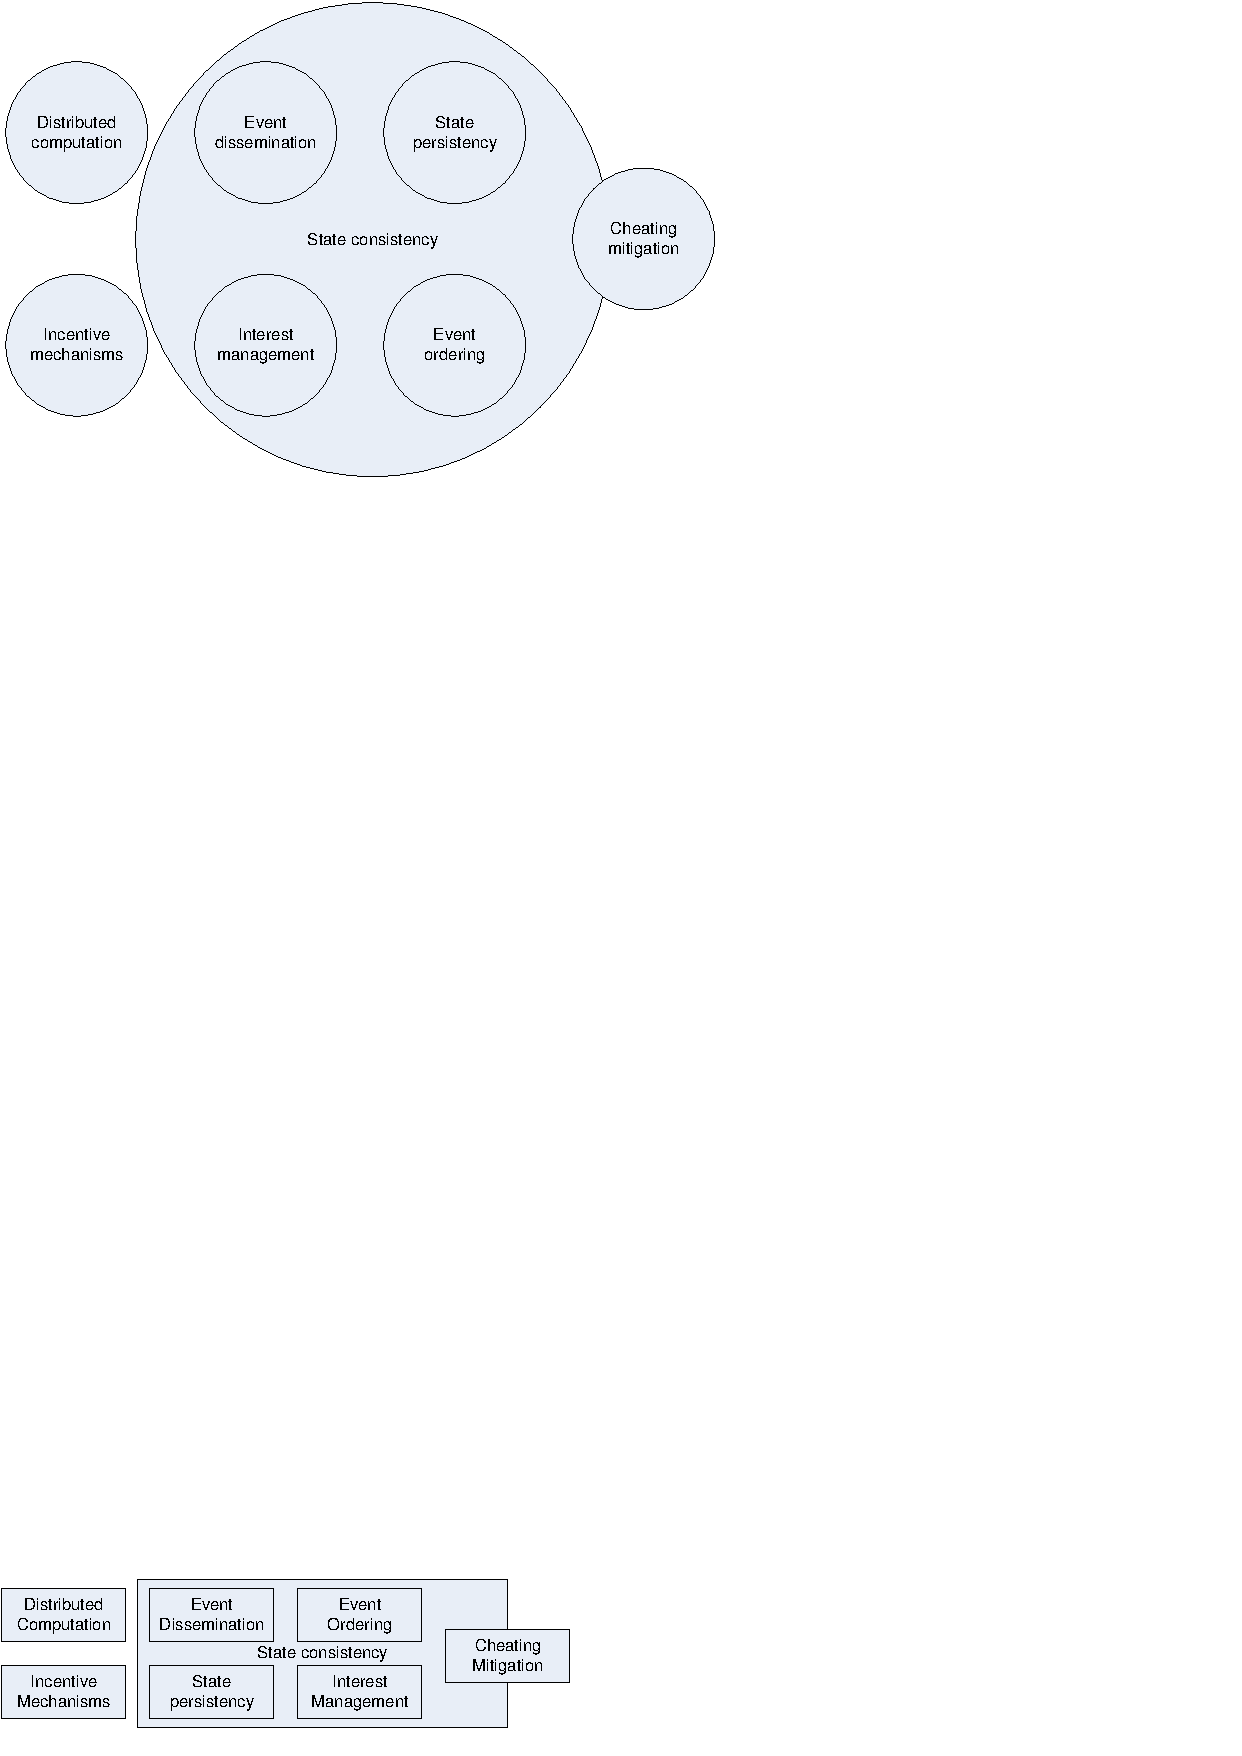
\includegraphics[clip=true, viewport=0cm 0cm 10cm 3cm, width=0.5\columnwidth]{Component_VEN}
 \caption{VEN diagram showing the relationship between different characteristics}
 \label{fig_component_ven}
\end{figure}
%
As shown in Figure \ref{fig_component_ven}, of the six challenges mentioned, Interest Management, Game Event Dissemination and Game State Persistency
all form part of State Consistency, with some aspects of Cheating Mitigation also a part of State Consistency. Also part of state consistency is
event ordering, which deals with how to ensure that the system remains causal \cite{GauthierDickey_low_latency_event_ordering}.

Key to designing an MMVE is to design its state consistency architecture. On a physical level, each computer that executes a virtual environment (VE) is executing a copy of the virtual environment. This is because a computer can only operate on what is stored in its primary memory. Because computers cannot access each other's primary memory banks, the necessity of multiple object copies is created.

A virtual environment can be characterised by its state. The \emph{environment state} (\emph{game state} when the environment is an online game) includes all positions, health and other attributes of all avatars, NPCs and other objects in the VE. The environment state consists of a collection of objects. An NPC as well as an immutable plant are both examples of objects that together make up the environment state.

When discussing how to segment VE state, it is sometimes easier to speak in terms of \emph{objects}, since they are separable. For the purposes of this work, objects are entities with both state and logic, which means they consume both storage space, as well as computing resources. Objects can also produce events, which should be sent to other objects. When this definition is used, NPC objects may be classified as a specific type of object, which forms part of the global game state.

The existence of multiple object copies necessitates an object consistency model. In MMVEs, each computer uses the information of the virtual environment, stored in memory, to display the virtual environment to the user. The user makes decisions based on what is displayed and the executed operations on the environment. These operations can effect change in the environment and this change has to be communicated to all other entities capable of interacting with the environment. The fact that users operate on a local version of the environment and that the environment should appear the same to all users requires state consistency mechanisms.

\section{Event-logic-update cycle}
\label{event_logic_update}

\subsection{Overview}

It is however impossible for multiple object states to always be consistent, because it takes time to send a message about an object update that has occurred. It is, therefore, not a good design to allow objects to be locally changed and those changes to then be communicated to other objects, because other objects may also have been locally changed in a way that would not allow for the change in the first object.

An example would be of one player in a virtual game world dealing five damage to another player with five health. When the damage is dealt, the target player is killed. If, however, the player drank a potion that gives it some health, the damage dealt by the first player would not kill him. The state of the player being dead and the player being alive is not possible at the same time.

To overcome this difficulty, a disconnect is introduced between the actions that can be performed on objects and the effect that the actions can have on objects. This is called the event-logic-update cycle \cite{}.

\emph{Events} are generated by objects and can be thought of as actions taken by agents, where agents can be humans or artificial intelligence (AI) scripts. These include casting a spell, using an item or walking.

\emph{Environment logic} is applied to events to determine what updates should be applied to the environment state. Environment logic is thus a ``think'' function, which determines how the environment should change as a result of an event. Another way to think about environment logic is to see it as the game rules.

A player casting a spell might cause another player's health to be reduced, her own health to be increased or a monster to spawn. When a player is walking, the logic will cause the player's position to update at the player's walking speed.

Environment logic communicates how the world should change via \emph{state updates}. State updates are the incremental changes that specify how the environment state should change.

An object exists in two forms: the authoritative object and the non-authoritative object. The state of the authoritative object is considered to be the true state or absolute state. Copies of the authoritative object can be made, but these copies are all non-authoritative objects. If a discrepancy occurs between an authoritative object and a non-authoritative object, the state of the authoritative object is considered to be the true state. The work of the consistency mechanism in the VE is to ensure that all non-authoritative object states follows the authoritative object state within a time frame that is reasonable for the particular VE and the particular type of object.

Authoritative objects are the objects traditionally housed on the server in the C/S based MMVEs. All clients obtain replicas of these objects and duplicate them locally in order to perform low latency computations. An example would be an NPC monster. When players perceive the monster in the virtual world, a duplicate of the NPC objects is sent to the user's computer for display purposes. When another player attacks the NPC, the change in health will be computed at the server and an update is then sent in order to ensure consistency between root and replica objects.

\subsection{General flow}
\label{general_flow}

\begin{figure}[htbp]
 \centering
 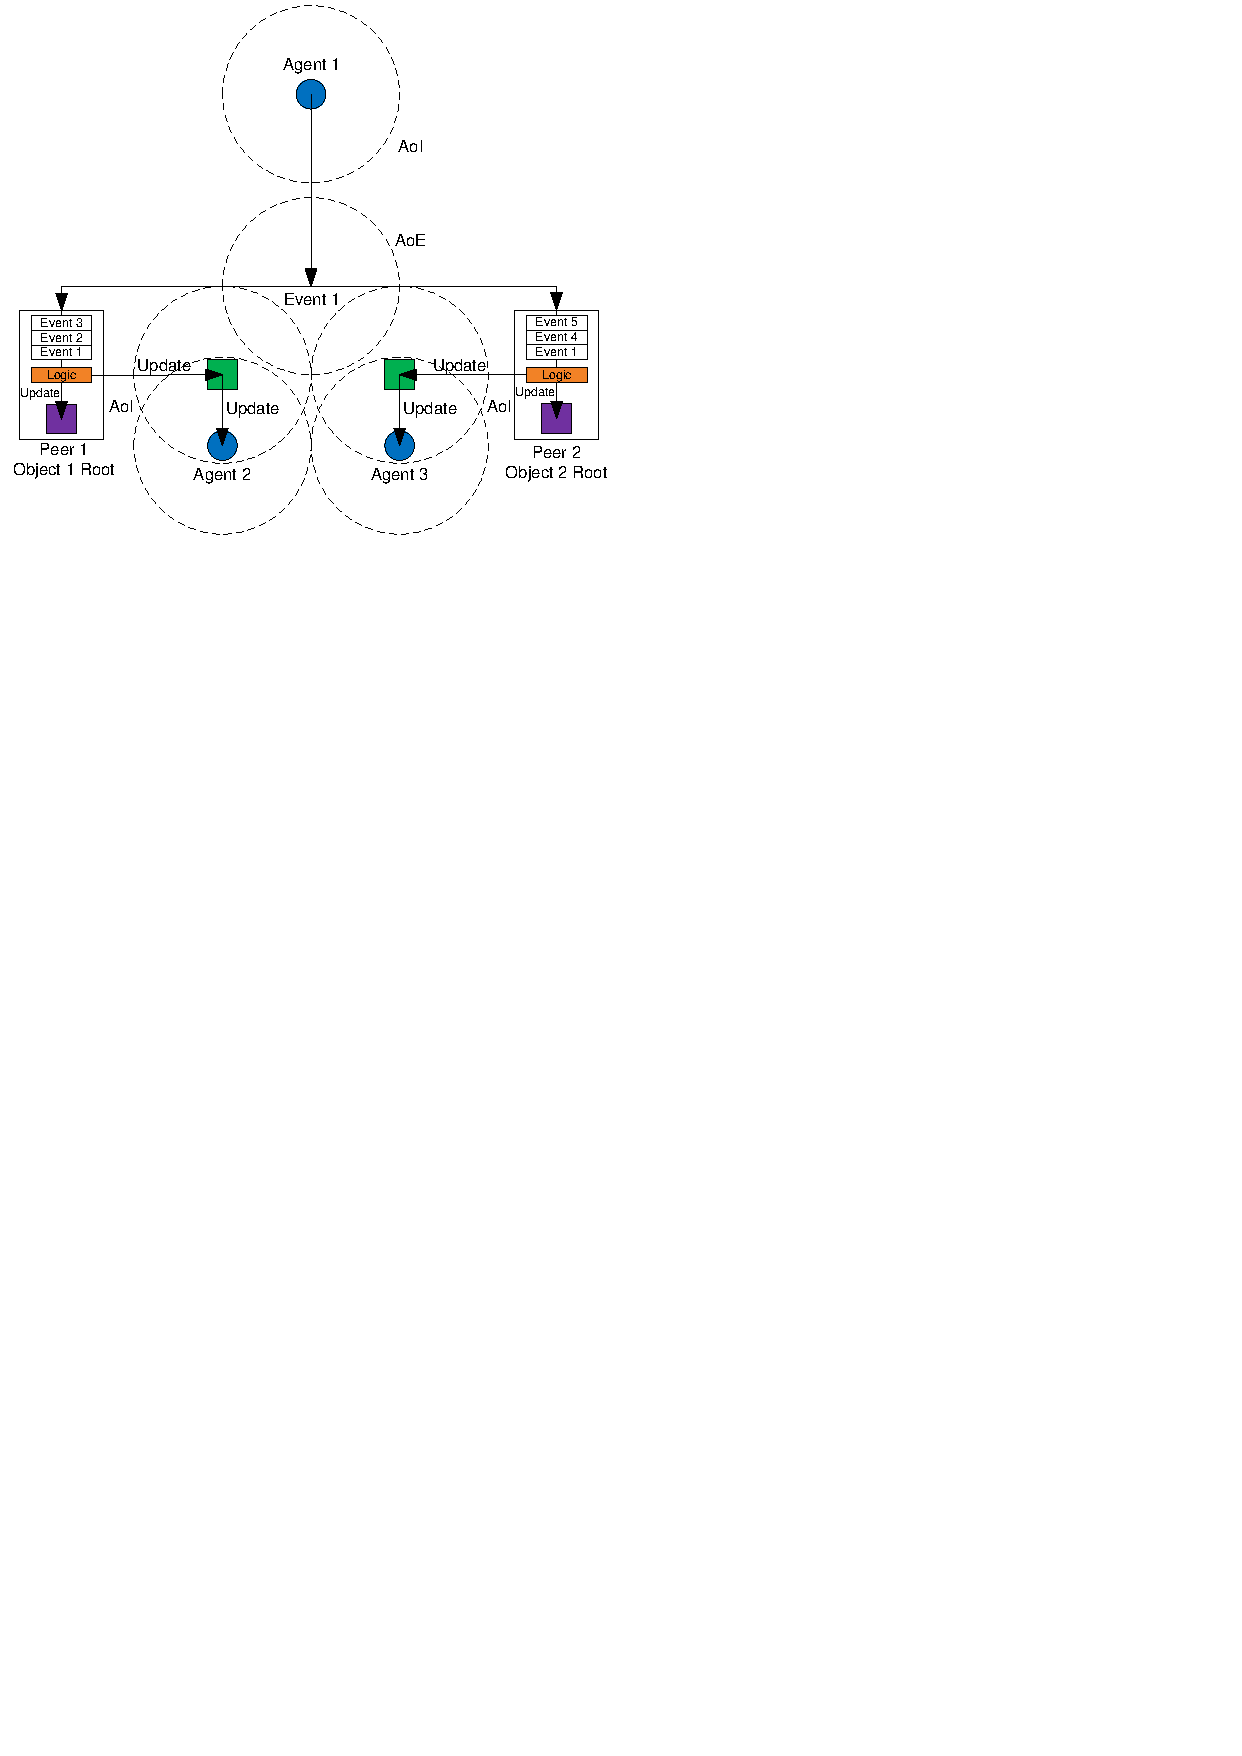
\includegraphics[clip=true, viewport=18mm 227mm 69mmm 292mm, width=0.6\textwidth]{generic_consistency_graphic}
 \caption{Graphic showing the flow of events and updates to achieve state consistency}
 \label{fig_event_update_flow_graphic}
\end{figure}

Figure \ref{fig_event_update_flow_graphic} depicts the flow of events and updates in response to the generation of an event by some agent. Agents are defined to be some form of intelligence that can interact with the virtual environment.

In Figure \ref{fig_event_update_flow_graphic}, Agent 1 generates Event 1 at the remote location shown. To maintain generality, events are defined to possess areas of effect (AoEs). An event's AoE determines which objects are in range to be potentially affected by an event. When an event's AoE encloses an object, that object is in range to be affected by the event. Whether the object is affected by the event, will be determined by the game logic.

In Figure \ref{fig_event_update_flow_graphic}, Event 1 affect Object 1. Event 1 is, therefore, sent to Object 1's root node, i.e. the peer housing the authoritative copy of Object 1. Determining which objects are affected by an event is termed \emph{event layer interest management}. Delivering the event to the root nodes of the affected object is termed \emph{event dissemination}.

When Event 1 arrives at Peer 1, containing Object 1, the event is placed in a event queue in an order based on the time each event occurred. The process of determining which order events have to be processed in is called \emph{event ordering}. Many events will be arriving at an object's root node from multiple agents simultaneously.

After event ordering has been performed, environment logic is applied to determine hoe a specific event will affect a specific object. To determine possible updates, that state of other objects might also have to be taken into account. An example is firing at a player through a wall. If the thickness of the wall determines how much damage is delivered to the player, the root node processing the damage to the player object will have to know the thickness of the wall.

When an event has been translated into a state update, the root object on the root node is updated. The new state of the object should also be communicated with all agents that can perceive the object in the virtual world. An object is perceived by an agent if the agent's area of interest (AoI) encompasses the object. Determining which agents should receive objext state updates is termed \emph{update layer interest management}. In the figure, Object 1 is perceived by Agent 2. Peer 1 therefore has to send an update to the peer housing agent 2. Delivering state updates to the affected agent peers is termed \emph{update dissemination}.

When the update is delivered to Agent 2, the local object state is updated and the object's new state is displayed to the agent to allow the agent to make decisions and, therefore, generate events based on the new object state.

\subsection{Generic event-update model}
\label{generic_event_update_model}

During the literature review process, many papers were reviewed that were said to deal with state consistency in P2P MMVEs \cite{}. These papers that were said to contain novel state consistency methods for P2P MMVEs, always only pertained to a specific part of the state consistency model and compared other papers related to the same part. All these papers improved on the various modules that make up a state consistency model, but failed to provide an overview of the bigger picture and how to place the work in the paper in the framework of a state consistency model.

Reviewing the various papers, it became evident that a higher level state consistency model is required to place all the work done in this field into perspective.

\begin{figure}[htbp]
 \centering
 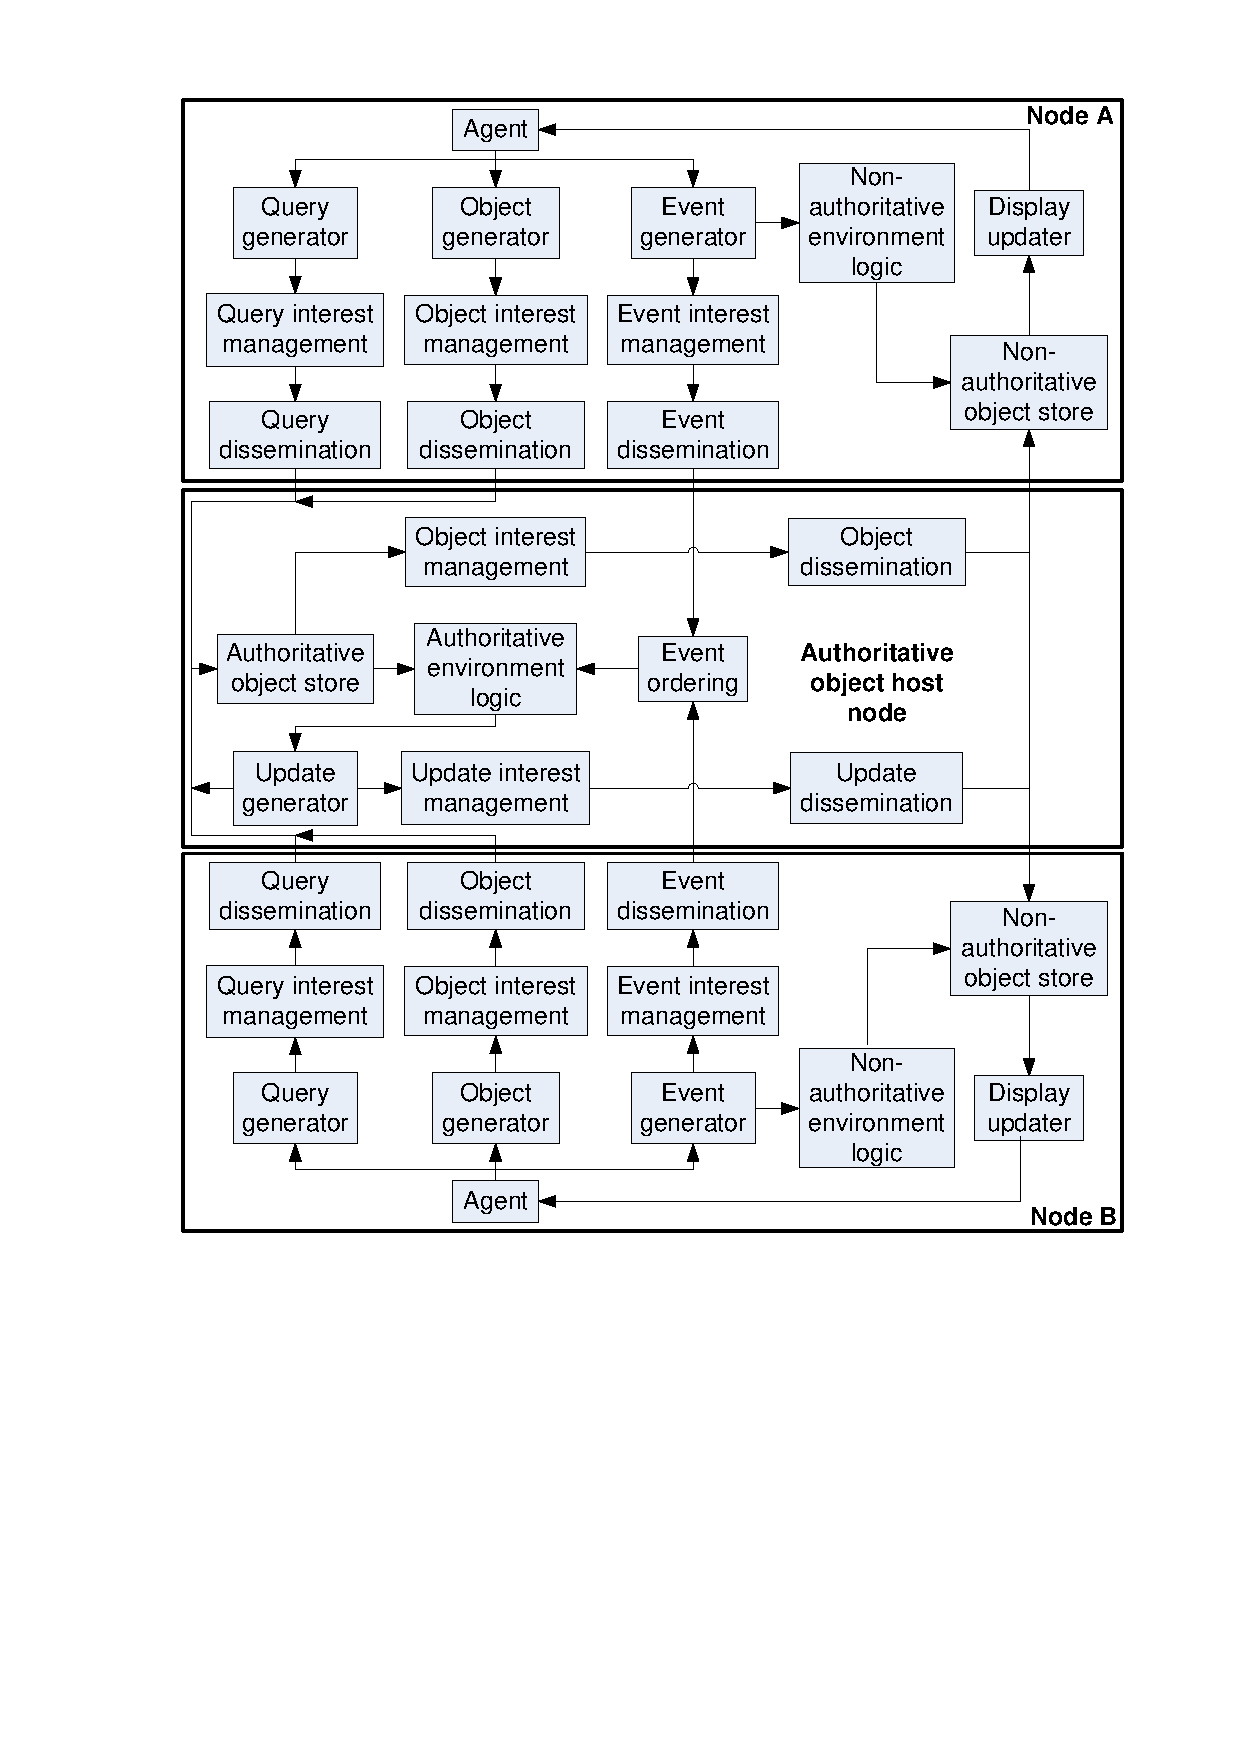
\includegraphics[clip=true, viewport=49mm 82mm 156mm 288mm, width=0.6\textwidth]{generic_consistency_flowdiagram}
 \caption{Flow diagram describing the event-update flow cycle and all steps required, from generating an event to delivering an update, to ensure object consistency.}
 \label{fig_event_update_flowdiagram}
\end{figure}

Figure \ref{fig_event_update_flowdiagram} shows the generic consistency flow diagram to ensure object state consistency. The agent, introduced in Section \ref{general_flow} is a player or AI script. An agent views the game world as the game displays is, makes some decisions on how it would like to influence the game world and then takes some action. The action of an agent is translated into an event.

Event layer interest management determines which objects will be affected and on which nodes these objects are housed. Event dissemination deals with how information is sent to peers after interest management determines which information should be sent. The first application of event dissemination for online games can be found in \cite{first_GED}.

The game logic is then applied to each received event and a corresponding update is generated. It is possible that the future state of an object might depend on the current state of the object, the received event and the state of some other object. The game logic might, therefore, require the states of other authoritative objects.

Storing authoritative data requires state management and state persistency. State management is the storage of objects in primary storage, while state persistency is the storage of the VE on secondary storage. State persistency does not have such rigorous responsiveness requirements as state management, as described in Section \ref{char_responsiveness}.

After the combination of event, object states and game logic, an event is generated. Update layer interest management determines which nodes require this update. These will typically be the nodes whose agents can perceive the object in the virtual environment and, therefore, stores local copies of the object.

Update dissemination will deliver the update to all local copies of the object. Multiple object updates may be generated for a single event. Any generated update may have to be delivered to multiple nodes that contain local copies of the object.

The flow diagram in Figure \ref{fig_event_update_flowdiagram} shows all actions that should be taken to ensure object consistency. This model is applicable to all known state consistency models for C/S as well as P2P network architectures.

What changes for the various architectures is where the root object is housed, and how the hosts of the root object are distributed. In a C/S system, all root objects are housed in the server. In a P2P architecture, root objects can be distributed on a number of peers or super peers, depending on the specific architecture. The various state consistency schemes for both C/S and P2P networks will be reviewed in the next sections.

\section{Classic consistency models}
\label{classic_models}

An overview of the two common models, currently used in computer games will be described. The models used in P2P MMVEs are all permutations of these two basic models. The two models are based on the two different network models. These are the fully distributed model, also called the event-based model \cite{p2p_cm_aoe}, and the C/S-based model, also called update-based model
\cite{unreal_networking}.

\subsection{Event-based (Fully distributed)}
\label{classic_event_based}

\begin{figure}[htbp]
\centering \subfloat[Event-based (fully distributed)]{\label{fig_p2p_cm}
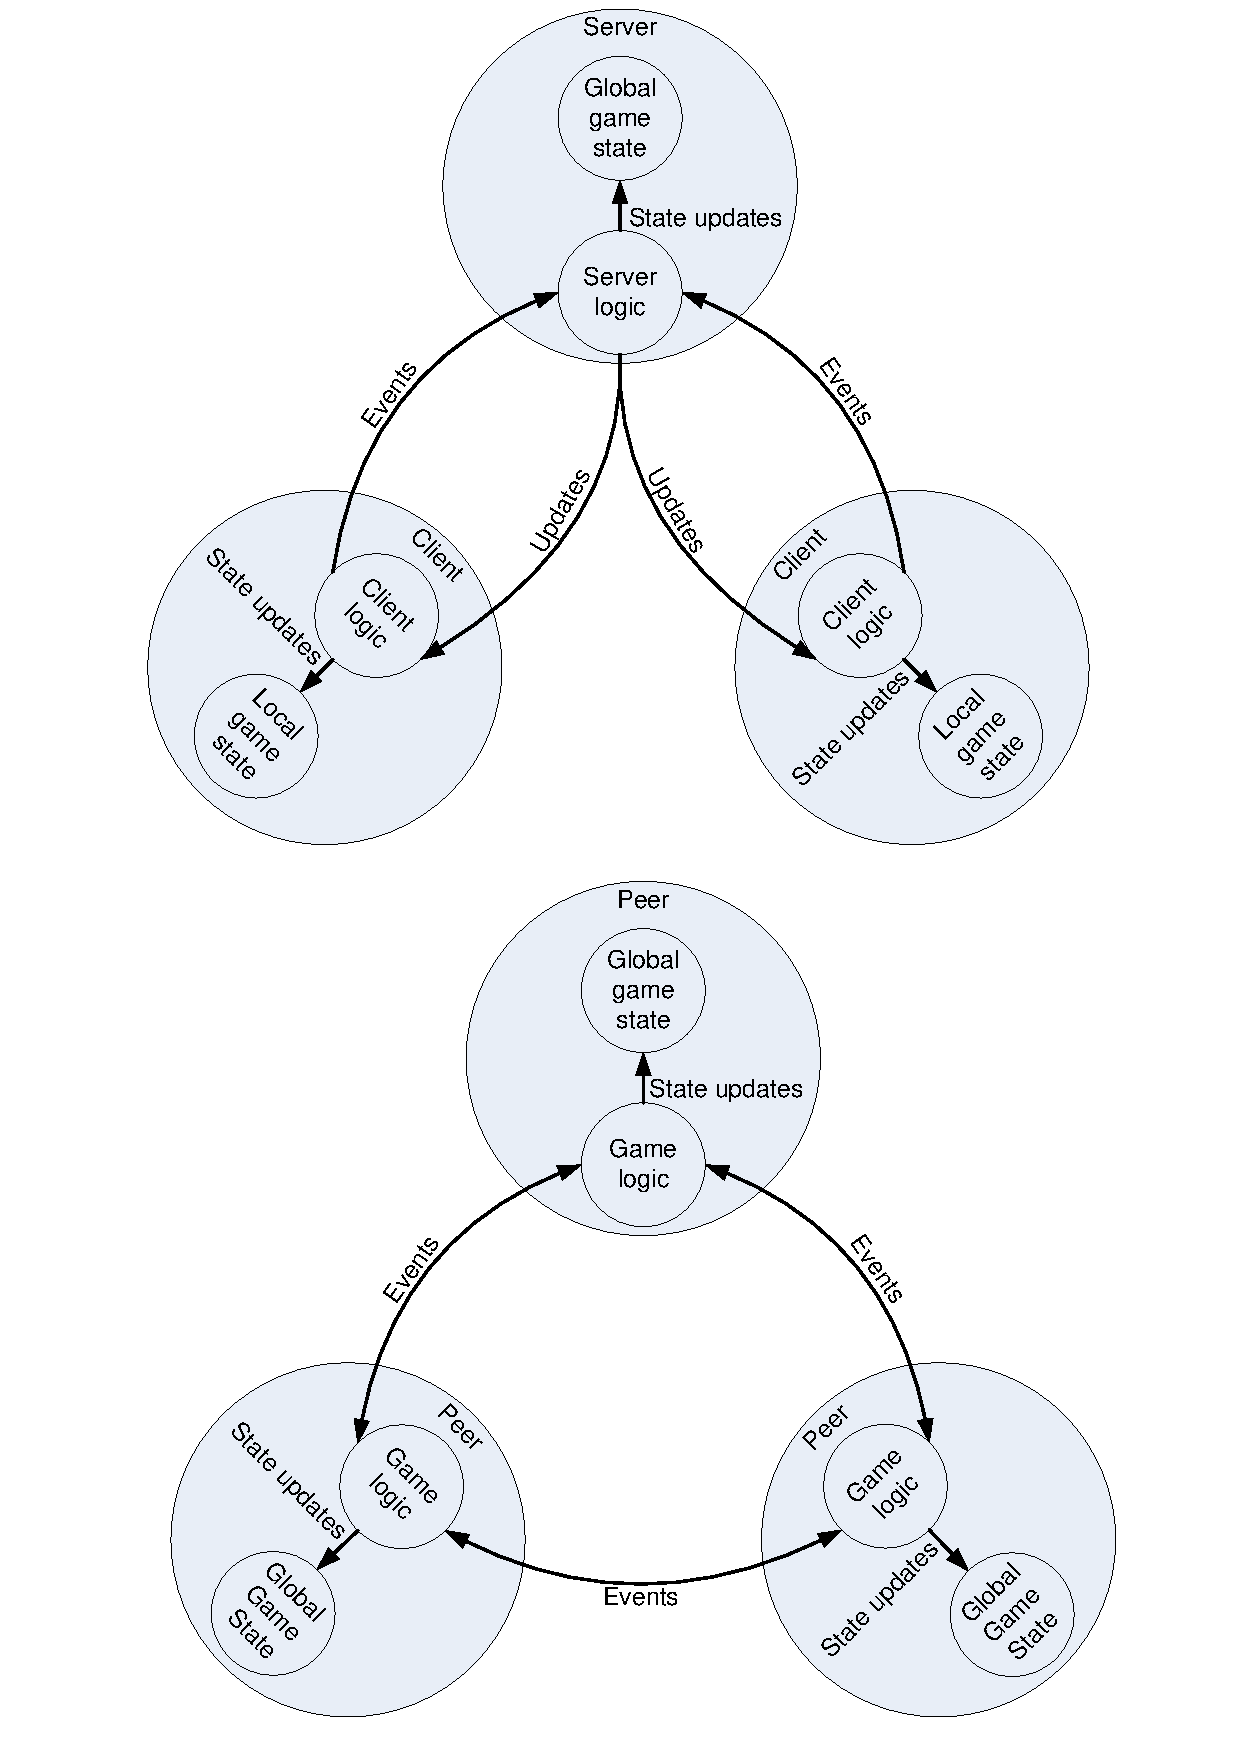
\includegraphics[clip=true, viewport= 2.5cm 0.5cm 19cm 15cm, width=0.5\columnwidth]{CS_P2P_CMs}}
 \subfloat[Update-based (client/server)]{\label{fig_cs_cm}
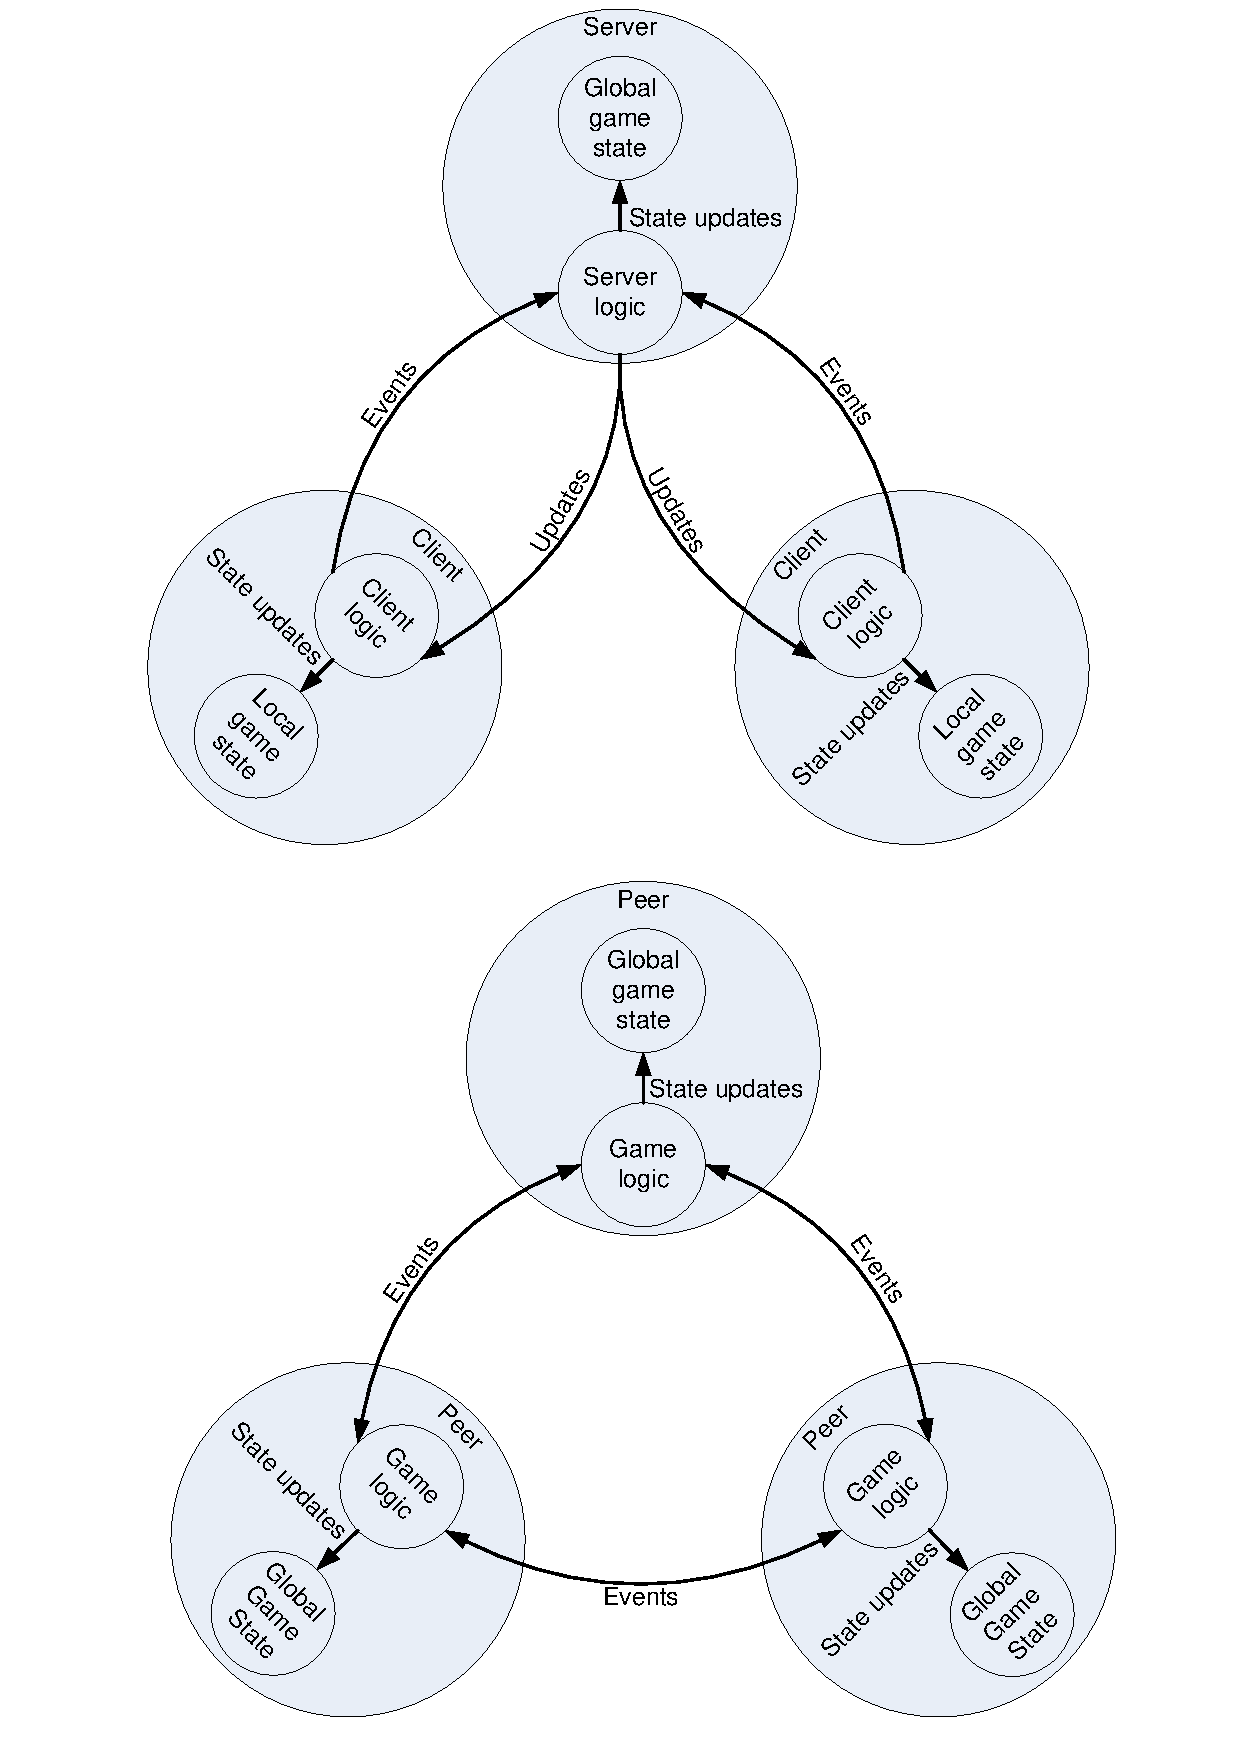
\includegraphics[clip=true, viewport= 2.5cm 15cm 19cm 30cm, width=0.5\columnwidth]{CS_P2P_CMs}}
\caption{Consistency models}
\end{figure}
%
Figure \ref{fig_p2p_cm} shows the fully distributed model. Any event that a peer generates is sent to all other peers. Each peer processes all events separately and updates its own game state accordingly. This consistency model is one where there exists multiple authoritative game states.

\subsubsection{Event generation and dissemination}

With reference to the generic flow diagram in Figure \ref{fig_event_update_flowdiagram}, user agents access the VE using peers in the fully connected network. Event generation occurs on peers.

Event layer interest management is trivial, since all peers receive all updates. Every peer, therefore, requires an up-to-date list of all other peers in the network. Event dissemination typically makes use of unicast to send all events to all peers.

\subsubsection{Event ordering}
The order in which events are received should be the same for all peers, otherwise the game states of different peers may become inconsistent.
Usually some kind of lockstep technique is used to solve this issue \cite{pessimistic_lock_step}. The issue with lockstep is that it reduces the latency to twice that of the peer with the highest latency.

Various techniques have been proposed that improves the latency by introducing some deadline before which all events should be submitted. An example of this is the New Event Ordering (NEO) technique \cite{cheat_proof_event_ordering}. This, however, makes it impossible for a player with high latency to play the game with anyone other than from her own continent.

An alternative to NEO is a P2P and C/S hybrid scheme, called the referee anti cheat scheme (RACS) \cite{cheating_taxonomy}. The scheme proposes referees, that are similar to the C/S network model, which allow for greater resistance to more types of cheats.

\subsubsection{Game logic}
Complete game logic is housed on every peer, since every peer must be able to translate any event into a state update. The game logic will determine a set of objects that will be affected by the received event and update the affected objects accordingly.

\subsubsection{Update generation and dissemination}

The game logic housed on every peer generates state updates. These state updates are only used to update the local copies of affected objects. Each peer is responsible for keeping its environment state up-to-date.

Update layer interest management and update dissemination is not required, since all affected peers will have received the event.

\subsubsection{Root object store}

The complete game state is stored on each peer.

\subsubsection{Advantages}
The event-based model works well for strategy games, and was implemented
in Age of Empires \cite{p2p_cm_aoe} and Starcraft \cite{starcraft_network_model}.

When latency issues are not present and all players possess reasonable
latencies, the event-based model can provide for an high-degree of responsiveness, because of no extra latency being added by a server and no extra server hop required for communications.

\subsubsection{Disadvantages}
The issue with the event-based model is that it is not scalable, since all peers should connect to all other peers and every event is transmitted to
everyone. This means that as $N$, the number of peers in the network increases, the traffic increases with a factor of $N^2$. The security issues of
the P2P network model, on which this consistency model is based, are also present. Slowdown is also experienced by all players if one player's
latency is below par, since the lockstep mechanism has to wait for all events to be received for that round to conclude.

\subsection{Update-based (C/S)}
\label{classic_update_based}

An alternative to the event-based model is the update-based model, shown in Figure \ref{fig_cs_cm}. This model is based on the C/S network model.

\subsubsection{Event generation and dissemination}
Actors control clients that are able to generate events. Event layer interest management is trivial, since all events are sent to the server, usually making use of a unicast event dissemination technique.

\subsubsection{Event ordering}
\label{cs_event_ordering}

Event ordering also has to be performed on the server-side, although not as critical as for the fully distributed model. If events are processed in different orders by different clients in the fully distributed model, the game states of the clients will start to diverge and no mechanism exists to merge the diverging states.

If event ordering is not performed in the update-based model, the server might execute some events out of the order in which they were generated. The game state will, however, remain consistent, since the server informs all clients of the game state as it calculates it.

\subsubsection{Game logic}
Most of the game logic is housed on the server. This allows for simplicity of design and increases system security, since the server can verify any actions performed by a client.

Some game logic might still be housed on the clients. This will typically be the handling of low risk events that don't require a high level on consistency, for example, movement updates.

\subsubsection{Update generation and dissemination}

The game logic generates states updates, which is used to update the server's authoritative game state and is also used to inform peers able to perceive the updated objects of the object's new state.

Update level interest management is required to determine which clients can perceive the updated objects. Unicast is then used as update dissemination technique to inform the affected clients of the updated object states.

\subsubsection{Root object store}
An authoritative global game state is housed on the server and a  non-authoritative local game state is housed on all clients for display purposes.

\subsubsection{Advantages}
The update-based model is used in many, if not all, MMVEs currently in operation. This includes games like World of Warcraft, Eve Online and Ultima Online, to name just a few.

This approach greatly assists with security, as clients cannot influence the state of any other clients and every client's state depends on updates
received from the server. The server state is also termed authoritative, because if there is a conflict, the server state is always the state to
which the system is expected to return. All the security advantages of the C/S model also apply to this consistency model.

Another reason why the update based model is successful is because it is more scalable then the fully distributed model. More hardware can be used to build a more powerful server, which can handle more clients.

\subsubsection{Disadvantages}

The main disadvantage is the high cost involved in obtaining and maintaining the computer clusters and server hardware, required to host the VE.

\section{P2P MMVE state consistency models}
\label{p2p_mmve_state_consistency}

An issue with the development of P2P MMVEs is that no complete consistency model has been proposed and implemented. Various schemes have been proposed to address the various challenges of P2P MMVE state consistency, but these have mostly occurred in isolation. Some of the proposed schemes will be reviewed. What should be noted is that the various areas of state consistency is quite modular, which might allow for the integration of the best schemes in each area into a comprehensive P2P MMVE state consistency model.

P2P MMVE schemes are based on one of the two classic consistency models described in Section \ref{classic_models}. Although it might seem that the fully distributed model is a better fit for P2P MMVE state consistency, this model has received less attention than the C/S model. The reason for this is partly because of the difficulties in getting the fully distributed model to scale. Usually the fully distributed model makes use of rounds, where players submit actions and all player actions are executed at the end of a round. In an MMVE with tens of thousands to millions of players, designing the round mechanism to remain scalable is a challenge. Rounds are required, because of the event ordering mechanism that ensures state consistency.

The C/S consistency architecture is applied to P2P MMVEs by distributing authoritative objects. Every authoritative object is maintained by a single node, that received all events for the object, applies the game logic and informs all nodes of the generated game updates. This effectively creates a C/S consistency model from the perspective of each authoritative object. An example of such a consistency model is the region-based model.

A region is usually created by segmenting the world and super peers act as regional servers to all peers in their region. Each super peer receives all events, handles all game logic and distributes updates to all peers in its region. The super peer also handles state management and persistency for its region, hosting NPCs, objects and persistent player data. Clients in the region only house copies of the regional objects and some client logic to update the local copies of objects.

\begin{figure}[htbp]
 \centering
 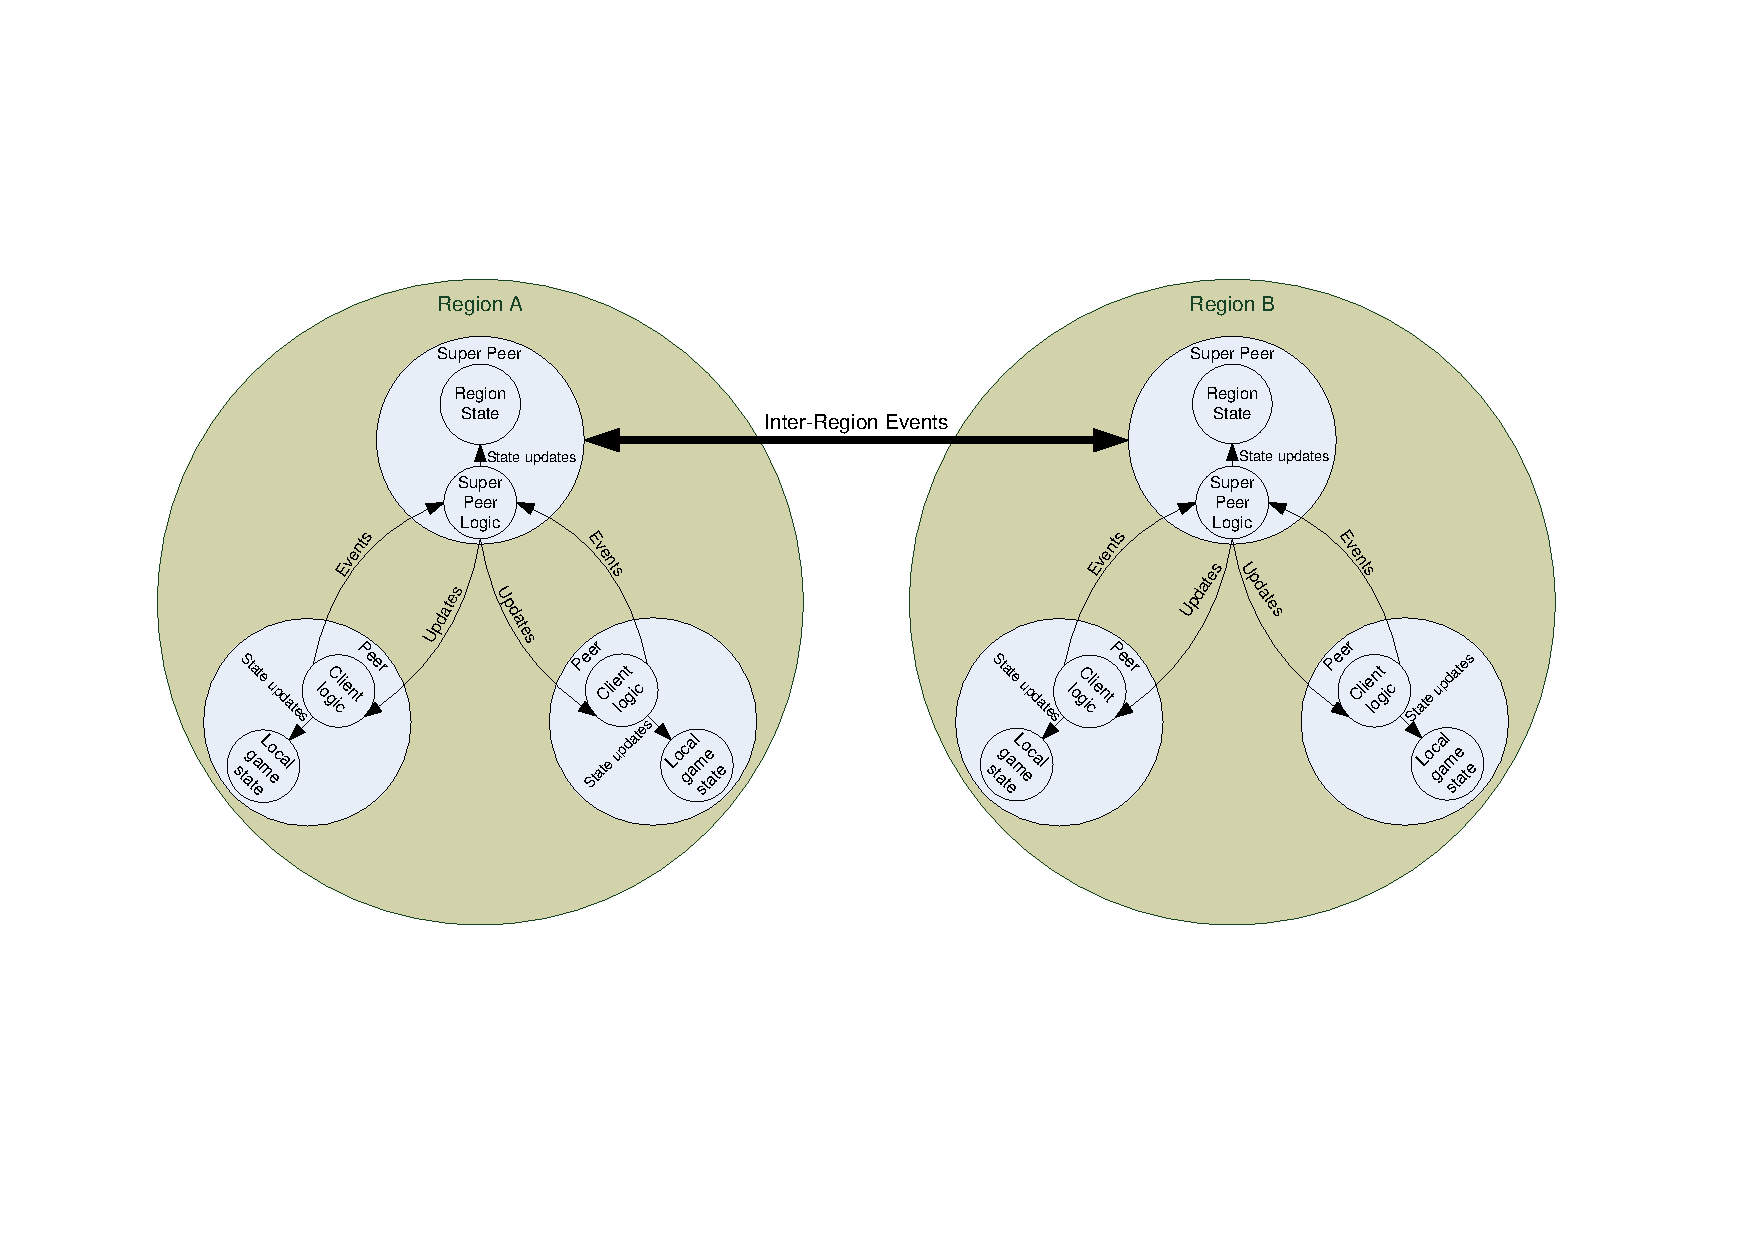
\includegraphics[clip=true, viewport=2cm 5cm 27cm 16.5cm, width=\textwidth]{region_based_CS_CM}
 \caption{Region-based Client/Server consistency model}
 \label{fig_cs_region_cm}
\end{figure}
%
The consistency model is depicted in Figure \ref{fig_cs_region_cm}. One can see that this approach is modelled on the update based model, but segmented into separate regions. The role of the server is here fulfilled by a super peer, which is a peer that is selected in some logical way, from the available set of peers and then promoted. Server selection in itself is a complex topic that has to deal with determining whether a peer has sufficient resources available and also whether the peer is trustworthy.

It should be noted that the overview presented here is only an overview of the different techniques and general trends present in the different areas
of peer-to-peer MMVEs. This overview does not presume to present an exhaustive list of papers in these areas, rather to place the topic of state persistency in context; to show readers how state persistency fits into the context of peer-to-peer games and to allow readers to distinguish between, for example, the topics of state persistency, interest management and event dissemination.

%Include the actual consistency models here. Region-based update-based, fully distributed

\subsection{Event generation and dissemination}

In P2P systems, each peer contains an agent that represents a player. Each peer can, therefore, generate events that have to be transmitted to the peers containing the authoritative objects affected by the generated event.

Recently, ALM and unicast techniques of event dissemination have become popular, depending on the grain of the event dissemination. ALM is used, instead of router level multicast, because of a lack of general support for this technology at the router level \cite{ip_multicast_deployment_issues}.

ALM is used for coarsely grained interest management techniques, while unicast is used for finely grained techniques. Unicast is not used for
coarsely grained techniques, because it is not scalable. For a network with $N$ nodes, $N^2$ messages are exchanges for every player action. ALM,
however, significantly increases the message latency in the system, because messages first have to be routed over a structured overlay network. ALM
is however preferred over unicast for large numbers of messages, because of the weak scalability of unicast.

An ALM scheme has recently been proposed, that sends updates to locations in the virtual world, rather than specific players
\cite{Ghaffari_Delaunay_churn_mobility}. This removes the need to first determine which nodes will be affected by an event, before the event may be
transmitted. Another ALM scheme proposed sends messages to the AoI neighbours, instead of to all the players in the region
\cite{Seeger_area_based_gossip_multicast}. This effectively implements a basic interest management scheme, where only neighbouring players can
receive events.

\subsection{Event ordering}

The presence and complexity of event ordering depends on the consistency architecture on which the P2P MMVE is based. In systems that use the update-based (C/S) model, no papers have addressed the issue of event ordering, since events delivered out of order will not lead to an inconsistent state, as discussed in Section \ref{cs_event_ordering}.

Where distributed architectures are proposed for P2P MMVEs, event ordering is of high importance. Designers of P2P MMVEs are making use of the same event ordering mechanisms used in the fully distributed model \cite{hybrid_storage1}.

To support a large number of players using an event-based model, event ordering with the concept of interest has been developed using N-trees \cite{GauthierDickey_ntrees}.

\subsection{Game logic}

In P2P architectures, the game logic for all objects have to be housed on all nodes, since any peer can be selected to store any object. The game logic itself is, therefore, usually distributed with the game along with the terrain and makes up the static game content. This is not to say that the game logic cannot change, but that a change in game logic will be in the form of a game update, which occurs while the game is off-line.

\subsection{Update generation and disseminiation}

In P2P MMVEs, update generation is done by the peer containing the authoritative object. When the peer receives an event, game logic is applied to generate an update. This update is then disseminated to all peers that contain agents that can perceive the object state to which the update pertains. This is similar to the update-based consistency model discussed in Section \ref{classic_update_based}.

\subsection{Update and event layer interest management}
\label{key_challenges_im}

Interest management has to occur both in the update and the event layer. For the event layer, the set of nodes has to be found, which house the root object affected by the generated event. For the update layer, the set of nodes has to be found which house the agents that will perceive an object update. What is common to both layers is that a message has to be sent to a subset of nodes with interest in the message and the interest management mechanism must determine what that subset is.

Thus far in P2P MMVE literature, little attention has been paid to whether the interest management in question is developed for the event layer or the update layer. Most discussions assume a layer and all the descriptions of the algorithm are based around the terminology of that layer. That is not to say that the algorithm itself might not be traversable to the other layer, just that this was never considered. Some interest management schemes for P2P MMVEs will not be reviewed along with the layers these schemes were designed for, but because of the similarities amongst the two layers, some schemes might be applicable to both.

Interest management is used to determine the smallest amount of information that a peer requires, in order to present an accurate representation of
the world to players. In consistency terms, it provides a means to determine which replica objects require updates of the root object. The idea is
not specific to P2P MMVEs and was already formally suggested in \cite{First_IM} and later with greater focus on a distributed environment in \cite{Whang_agent_based_IM}. Extensive research has been done into solving AoI problems and a comparison of techniques can be found in
\cite{Boulanger_IM_compare} and \cite{IM_and_ED_survey_Krause}.

The main idea is that a player has a limited visual range and area around the player in which it can interact with objects. The player requires
update information of all objects in this area, called the player's Area of Interest (AoI). AoI calculations also rely on the fact the a player's
direction and velocity of movement cannot change instantaneously and are bounded in magnitude.

Extensive research has been done into solving AoI problems and a comparison of techniques can be found in \cite{Boulanger_IM_compare} and
\cite{IM_and_ED_survey_Krause}. The solutions range from aura/nimbus \cite{Benford_spatial_IM} to publish/subscribe  \cite{mercury_publish_subscribe} to Voronoi based models \cite{Hu_voronoi_IM},  \cite{Buyukkaya_voronoi_state_management} to hybrid models \cite{hybrid_IM}, \cite{MOPAR}, \cite{fan_mediator_paper}.

Generally, interest management solutions can be divided into coarsely or finely grained solutions, although the hybrid models, especially MOPAR, seem to have gained greater popularity because they seem to have all the benefits of the two solutions and little of the drawbacks \cite{MOPAR}. MOPAR has
been shown to perform better than either a finely grained technique or a coarsely grained technique.

Coarsely grained solutions usually divide the game world into multiple regions and when a player enters a region, it subscribes to that region's
events. This is called the region-based publish subscribe model \cite{Fan_deisgn_issues_p2p}. All players in the region then receive the region's events, even for players not in their AoI.

Finely grained techniques create groups of players from their AoI. Groups of interacting players directly exchange information, so all players
only receive information that is relevant to them. This has been termed the spatial model \cite{Fan_deisgn_issues_p2p}. The grain of the solution in
turn determines the type of event dissemination that should be used, as described later in this section.

Another example of finely grained interest management was presented in \cite{IM_frontier_sets}. Interest management was achieved by making use of
frontier sets and this was implemented in Quake 3. By using Frontier Sets, it is possible to describe an area in which a player may move, where no
other players will require updates of that movement. Conversely, a set of other players that require movement updates from a specific player is also
given by the frontier set.

MOPAR partitions the game world into hexagonal regions and appoints ``home'' nodes to act as bootstrap nodes for each region. A home node of a region
is that node whose ID is the closest match the the region ID. This allows any node to find the home node for a region. A master node is then selected
for every region, whose function it is to inform slave nodes of new neighbours. All slaves nodes in a region register at their region's master node.

Slave nodes send direction and velocity updates to their masters. Masters communicate directly with other masters if a node is about to enter their
region. Masters inform their slaves of a new neighbour. Slaves communicate directly with each other, once identified by a master.

\subsection{Root object store}


In a recently completed PhD on the subject of P2P MMVEs, Lu Fan had this to say about state persistency: ``Game state persistency is a major challenge for P2P MMVEs as existing P2P storage infrastructures are designed to support file sharing, and seldom fulfil the performance and security requirements of a MMVE. \ldots the persistency area is still immature with many problems waiting to be investigated.'' \cite{Fan_phd}.

State persistency is treated as a sub domain of state consistency, in that state persistency models define where and how the root or authoritive
objects are stored. It is assumed that replica objects are always stored in the primary memory of the clients that immediately require the
information contained in the root object.

The issue of game state persistency in P2P MMVEs is the focus of this paper and the remainder of the paper will deal exclusively with this subject.
However, before the different storage types are reviewed, some classic C/S models are presented for comparison with the fully distributed model.

\section{Conclusion}

This chapter introduced the event-update consistency model that is mostly used in MMVE. From the literature reviewed, a generic process was developed that will ensure state consistency. Classic state consistency models were introduced and it was shown how these models relate to the generic state consistency process. After this, state consistency for P2P MMVEs were described. It was shown how the models used are all based on the classic consistency models. Some research into every area of P2P MMVE state consistency was discussed to enable the reader to place the work done here, into perspective.

In this chapter it was shown that the field of P2P MMVE state consistency is a growing one, already containing many significant contributions. But is was also shown that there is still much room for improvement on how we think about state management and state persistency and that there are still many open questions in these fields.